% Raportul de proiect DCTC: scheletul echipei (Overleaf, compilator pdfLaTeX).
% Ce completați: textele din parantezele drepte roșii, \decompletat{...}; la final nu mai rămâne niciunul.
% Nu redenumiți main.tex, refs.bib și folderul figures/; numele fișierelor: litere mici, fără spații și diacritice.

\documentclass[11pt,a4paper]{article}

% Pachetele (explicate în cursul 4, capitolul 5)
\usepackage[T1]{fontenc}         % diacriticele ă, â, î, ș, ț și despărțirea în silabe
\usepackage[romanian]{babel}     % „Figura”, „Tabela”, „Bibliografie”, regulile limbii române
\usepackage{lmodern}             % fontul Latin Modern, clar și pe ecran
\usepackage[margin=2.5cm]{geometry}
\usepackage{amsmath}             % formule: equation, align
\usepackage{graphicx}            % figuri: \includegraphics
\usepackage{booktabs}            % tabele: \toprule, \midrule, \bottomrule
\usepackage{xcolor}
\usepackage[numbers]{natbib}   % citări numerotate [1]; adresele web și DOI-urile în bibliografie
\usepackage[hidelinks]{hyperref} % link-uri; se încarcă ultimul

% Marcajul câmpurilor de completat (îl ștergeți pe măsură ce completați)
\newcommand{\decompletat}[1]{\textcolor{red}{[#1]}}

\title{\decompletat{Titlul studiului, o întrebare sau o afirmație scurtă}}
\author{\decompletat{Prenume Nume} \and \decompletat{Prenume Nume} \and \decompletat{Prenume Nume}\\[4pt]
  \small Echipa \decompletat{numele echipei}, \emph{Dezvoltare colaborativă și tehnologii cloud}}
\date{\today}

\begin{document}

\maketitle

\begin{abstract}
\decompletat{Trei--cinci propoziții: întrebarea studiului, datele folosite, metoda, rezultatul principal.
Rezumatul se scrie la final.}
\end{abstract}

\section{Introducere}
\label{sec:introducere}

\decompletat{Contextul temei și de ce contează; întrebarea studiului, formulată exact ca în README;
ce urmează în raport. La T4: cel puțin 200 de cuvinte și cel puțin două citări din bibliografie.}

\section{Date și metodă}
\label{sec:date}

Datele provin din \decompletat{sursa}~\cite{exemplu_set_date}.
\decompletat{Ce conține setul de date (perioada, unitatea, coloanele folosite), cum a fost descărcat
și cum a fost curățat.}

Indicatorul principal este \decompletat{numele indicatorului}, calculat cu relația
\begin{equation}
  r_t = \frac{x_t - x_{t-1}}{x_{t-1}} \cdot 100,
  \label{eq:indicator}
\end{equation}
unde $x_t$ este \decompletat{semnificația lui $x_t$}, iar $r_t$ este \decompletat{semnificația lui $r_t$}.
\decompletat{Înlocuiți relația~\eqref{eq:indicator} cu formula specifică temei voastre.}

\section{Rezultate}
\label{sec:rezultate}

Tabela~\ref{tab:rezumat} rezumă \decompletat{ce rezumă}, iar Figura~\ref{fig:principala} arată
\decompletat{ce arată}.

\begin{table}[htbp]
  \centering
  \caption{\decompletat{Titlul tabelei} (valori ilustrative).}
  \label{tab:rezumat}
  \begin{tabular}{lrr}
    \toprule
    \decompletat{Categoria} & \decompletat{Indicatorul 1} & \decompletat{Indicatorul 2} \\
    \midrule
    A & 12,4 & 3,1 \\
    B & 10,8 & 2,7 \\
    C & 9,5  & 2,2 \\
    \bottomrule
  \end{tabular}
\end{table}

\begin{figure}[htbp]
  \centering
  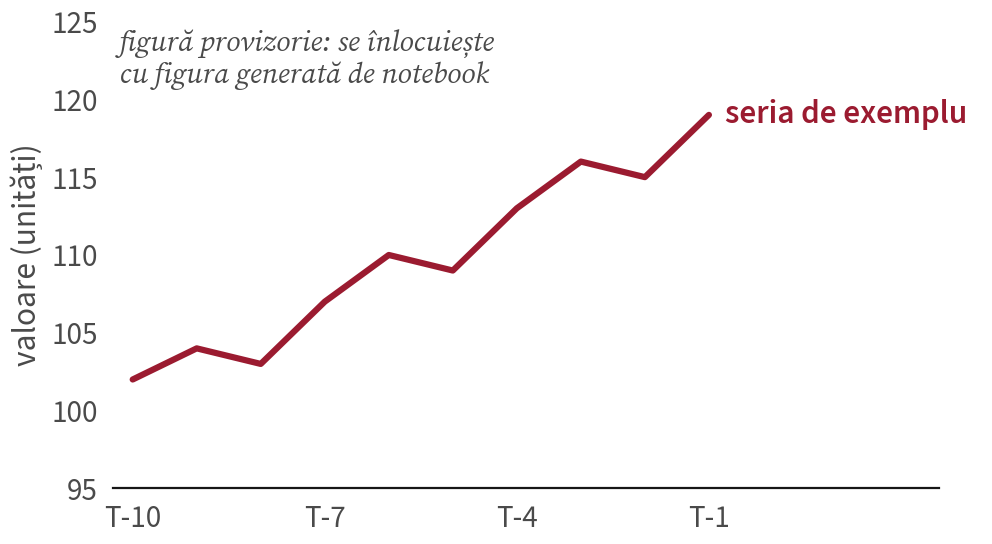
\includegraphics[width=0.85\textwidth]{figures/figura-exemplu.png}
  \caption{\decompletat{Titlul figurei: ce, unde, când; sursa datelor}.}
  \label{fig:principala}
\end{figure}

\decompletat{Interpretarea rezultatelor: ce se vede în tabelă și în figură, cu valori concrete.}

\section{Concluzii}
\label{sec:concluzii}

\decompletat{Răspunsul la întrebarea studiului, limitele analizei, ce s-ar putea face mai departe.}

% Bibliografia: intrările din refs.bib (exportate din Zotero, cursul 5), citate în text cu \cite{...}.
% Stilul unsrtnat le numerotează în ordinea primei citări și afișează URL-urile și DOI-urile.
\bibliographystyle{unsrtnat}
\bibliography{refs}

\section*{Declarație privind utilizarea instrumentelor AI}

\decompletat{Am folosit <instrument> pentru <scop> la <secțiune>; am verificat rezultatul prin <metodă>.
Sau: Nu am folosit instrumente AI.}

\section*{Contribuția fiecărui membru}

\begin{itemize}
  \item \decompletat{Prenume Nume}: \decompletat{ce a scris sau a făcut}.
  \item \decompletat{Prenume Nume}: \decompletat{ce a scris sau a făcut}.
  \item \decompletat{Prenume Nume}: \decompletat{ce a scris sau a făcut}.
\end{itemize}

\end{document}
